\documentclass[1p]{elsarticle_modified}
%\bibliographystyle{elsarticle-num}

%\usepackage[colorlinks]{hyperref}
%\usepackage{abbrmath_seonhwa} %\Abb, \Ascr, \Acal ,\Abf, \Afrak
\usepackage{amsfonts}
\usepackage{amssymb}
\usepackage{amsmath}
\usepackage{amsthm}
\usepackage{scalefnt}
\usepackage{amsbsy}
\usepackage{kotex}
\usepackage{caption}
\usepackage{subfig}
\usepackage{color}
\usepackage{graphicx}
\usepackage{xcolor} %% white, black, red, green, blue, cyan, magenta, yellow
\usepackage{float}
\usepackage{setspace}
\usepackage{hyperref}

\usepackage{tikz}
\usetikzlibrary{arrows}

\usepackage{multirow}
\usepackage{array} % fixed length table
\usepackage{hhline}

%%%%%%%%%%%%%%%%%%%%%
\makeatletter
\renewcommand*\env@matrix[1][\arraystretch]{%
	\edef\arraystretch{#1}%
	\hskip -\arraycolsep
	\let\@ifnextchar\new@ifnextchar
	\array{*\c@MaxMatrixCols c}}
\makeatother %https://tex.stackexchange.com/questions/14071/how-can-i-increase-the-line-spacing-in-a-matrix
%%%%%%%%%%%%%%%

\usepackage[normalem]{ulem}

\newcommand{\msout}[1]{\ifmmode\text{\sout{\ensuremath{#1}}}\else\sout{#1}\fi}
%SOURCE: \msout is \stkout macro in https://tex.stackexchange.com/questions/20609/strikeout-in-math-mode

\newcommand{\cancel}[1]{
	\ifmmode
	{\color{red}\msout{#1}}
	\else
	{\color{red}\sout{#1}}
	\fi
}

\newcommand{\add}[1]{
	{\color{blue}\uwave{#1}}
}

\newcommand{\replace}[2]{
	\ifmmode
	{\color{red}\msout{#1}}{\color{blue}\uwave{#2}}
	\else
	{\color{red}\sout{#1}}{\color{blue}\uwave{#2}}
	\fi
}

\newcommand{\Sol}{\mathcal{S}} %segment
\newcommand{\D}{D} %diagram
\newcommand{\A}{\mathcal{A}} %arc


%%%%%%%%%%%%%%%%%%%%%%%%%%%%%5 test

\def\sl{\operatorname{\textup{SL}}(2,\Cbb)}
\def\psl{\operatorname{\textup{PSL}}(2,\Cbb)}
\def\quan{\mkern 1mu \triangleright \mkern 1mu}

\theoremstyle{definition}
\newtheorem{thm}{Theorem}[section]
\newtheorem{prop}[thm]{Proposition}
\newtheorem{lem}[thm]{Lemma}
\newtheorem{ques}[thm]{Question}
\newtheorem{cor}[thm]{Corollary}
\newtheorem{defn}[thm]{Definition}
\newtheorem{exam}[thm]{Example}
\newtheorem{rmk}[thm]{Remark}
\newtheorem{alg}[thm]{Algorithm}

\newcommand{\I}{\sqrt{-1}}
\begin{document}

%\begin{frontmatter}
%
%\title{Boundary parabolic representations of knots up to 8 crossings}
%
%%% Group authors per affiliation:
%\author{Yunhi Cho} 
%\address{Department of Mathematics, University of Seoul, Seoul, Korea}
%\ead{yhcho@uos.ac.kr}
%
%
%\author{Seonhwa Kim} %\fnref{s_kim}}
%\address{Center for Geometry and Physics, Institute for Basic Science, Pohang, 37673, Korea}
%\ead{ryeona17@ibs.re.kr}
%
%\author{Hyuk Kim}
%\address{Department of Mathematical Sciences, Seoul National University, Seoul 08826, Korea}
%\ead{hyukkim@snu.ac.kr}
%
%\author{Seokbeom Yoon}
%\address{Department of Mathematical Sciences, Seoul National University, Seoul, 08826,  Korea}
%\ead{sbyoon15@snu.ac.kr}
%
%\begin{abstract}
%We find all boundary parabolic representation of knots up to 8 crossings.
%
%\end{abstract}
%\begin{keyword}
%    \MSC[2010] 57M25 
%\end{keyword}
%
%\end{frontmatter}

%\linenumbers
%\tableofcontents
%
\newcommand\colored[1]{\textcolor{white}{\rule[-0.35ex]{0.8em}{1.4ex}}\kern-0.8em\color{red} #1}%
%\newcommand\colored[1]{\textcolor{white}{ #1}\kern-2.17ex	\textcolor{white}{ #1}\kern-1.81ex	\textcolor{white}{ #1}\kern-2.15ex\color{red}#1	}

{\Large $\underline{12a_{0438}~(K12a_{0438})}$}

\setlength{\tabcolsep}{10pt}
\renewcommand{\arraystretch}{1.6}
\vspace{1cm}\begin{tabular}{m{100pt}>{\centering\arraybackslash}m{274pt}}
\multirow{5}{120pt}{
	\centering
	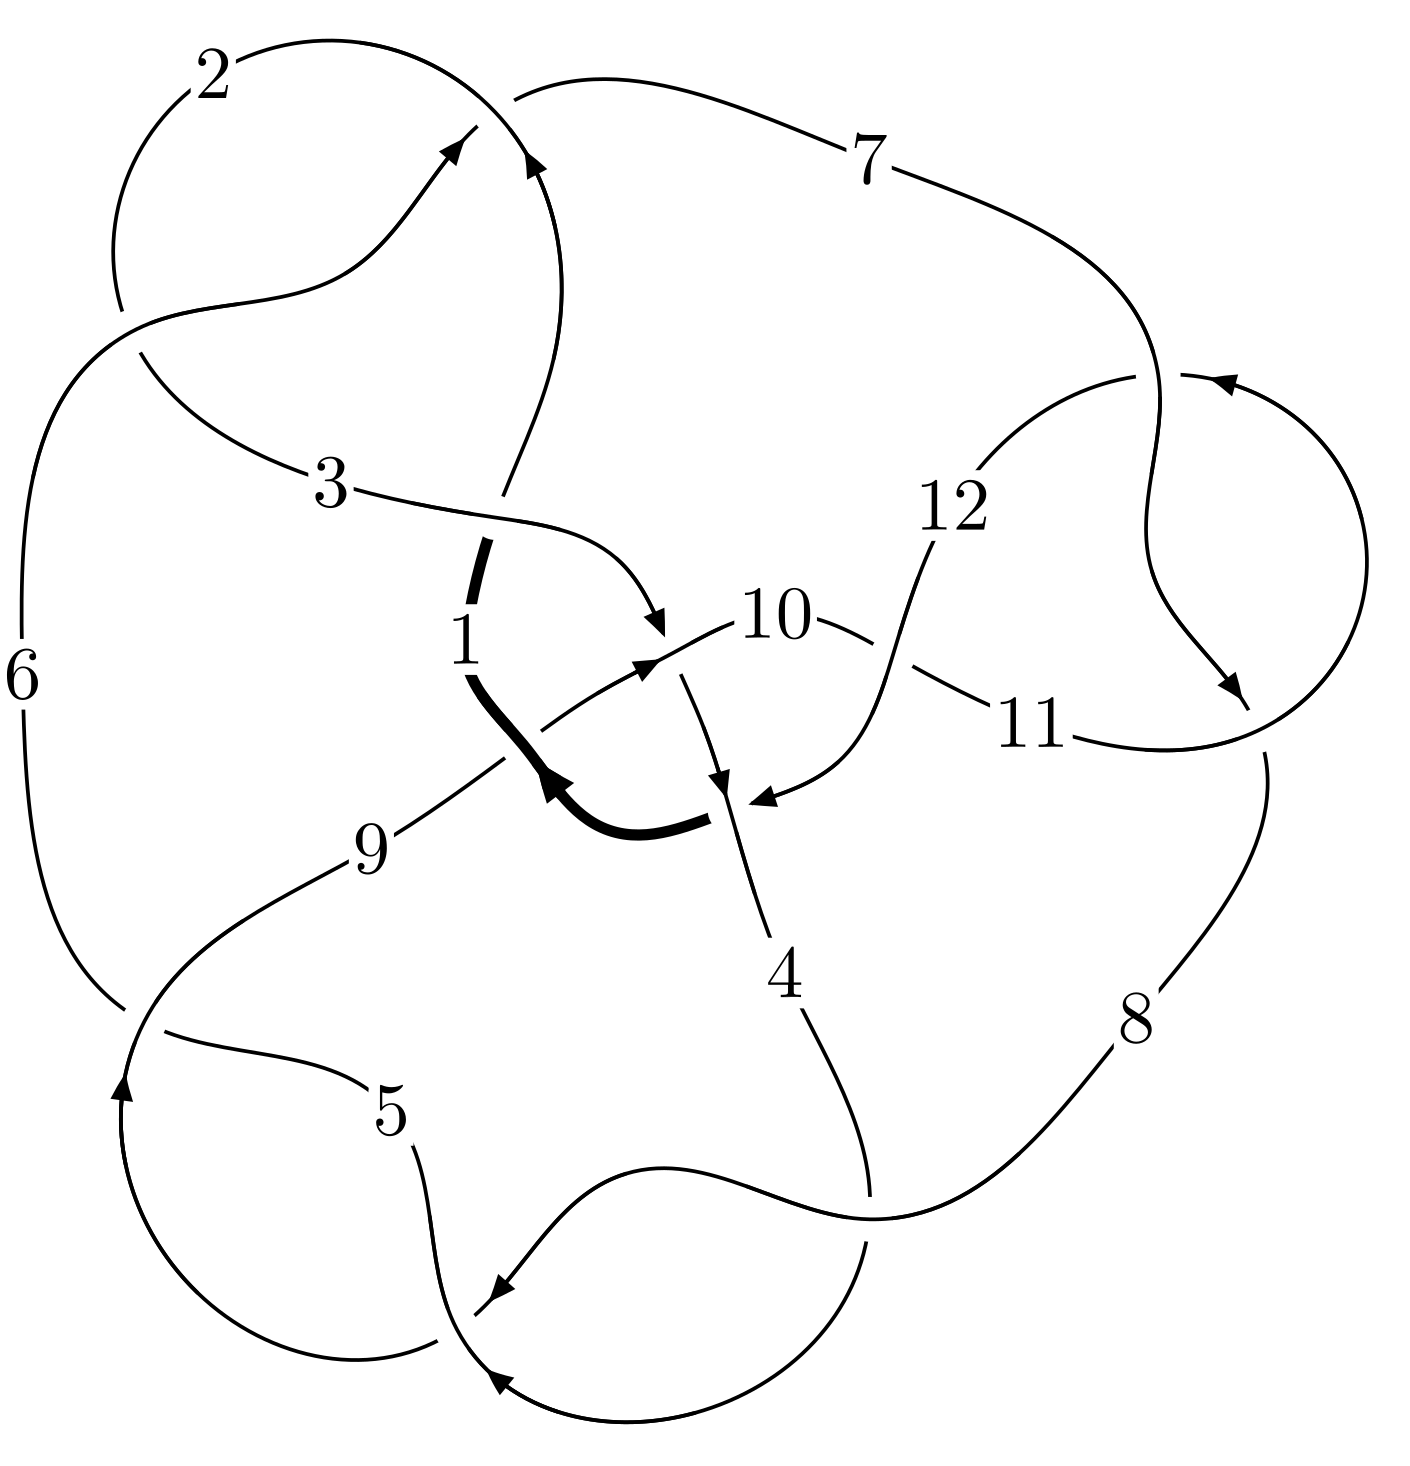
\includegraphics[width=112pt]{../../../GIT/diagram.site/Diagrams/png/1239_12a_0438.png}\\
\ \ \ A knot diagram\footnotemark}&
\allowdisplaybreaks
\textbf{Linearized knot diagam} \\
\cline{2-2}
 &
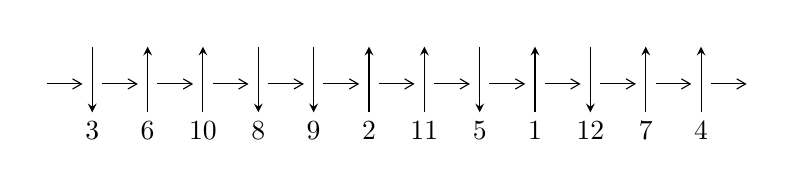
\begin{tikzpicture}[x=20pt, y=17pt]
	% nodes
	\node (C0) at (0, 0) {};
	\node (C1) at (1, 0) {};
	\node (C1U) at (1, +1) {};
	\node (C1D) at (1, -1) {3};

	\node (C2) at (2, 0) {};
	\node (C2U) at (2, +1) {};
	\node (C2D) at (2, -1) {6};

	\node (C3) at (3, 0) {};
	\node (C3U) at (3, +1) {};
	\node (C3D) at (3, -1) {10};

	\node (C4) at (4, 0) {};
	\node (C4U) at (4, +1) {};
	\node (C4D) at (4, -1) {8};

	\node (C5) at (5, 0) {};
	\node (C5U) at (5, +1) {};
	\node (C5D) at (5, -1) {9};

	\node (C6) at (6, 0) {};
	\node (C6U) at (6, +1) {};
	\node (C6D) at (6, -1) {2};

	\node (C7) at (7, 0) {};
	\node (C7U) at (7, +1) {};
	\node (C7D) at (7, -1) {11};

	\node (C8) at (8, 0) {};
	\node (C8U) at (8, +1) {};
	\node (C8D) at (8, -1) {5};

	\node (C9) at (9, 0) {};
	\node (C9U) at (9, +1) {};
	\node (C9D) at (9, -1) {1};

	\node (C10) at (10, 0) {};
	\node (C10U) at (10, +1) {};
	\node (C10D) at (10, -1) {12};

	\node (C11) at (11, 0) {};
	\node (C11U) at (11, +1) {};
	\node (C11D) at (11, -1) {7};

	\node (C12) at (12, 0) {};
	\node (C12U) at (12, +1) {};
	\node (C12D) at (12, -1) {4};
	\node (C13) at (13, 0) {};

	% arrows
	\draw[->,>={angle 60}]
	(C0) edge (C1) (C1) edge (C2) (C2) edge (C3) (C3) edge (C4) (C4) edge (C5) (C5) edge (C6) (C6) edge (C7) (C7) edge (C8) (C8) edge (C9) (C9) edge (C10) (C10) edge (C11) (C11) edge (C12) (C12) edge (C13) ;	\draw[->,>=stealth]
	(C1U) edge (C1D) (C2D) edge (C2U) (C3D) edge (C3U) (C4U) edge (C4D) (C5U) edge (C5D) (C6D) edge (C6U) (C7D) edge (C7U) (C8U) edge (C8D) (C9D) edge (C9U) (C10U) edge (C10D) (C11D) edge (C11U) (C12D) edge (C12U) ;
	\end{tikzpicture} \\
\hhline{~~} \\& 
\textbf{Solving Sequence} \\ \cline{2-2} 
 &
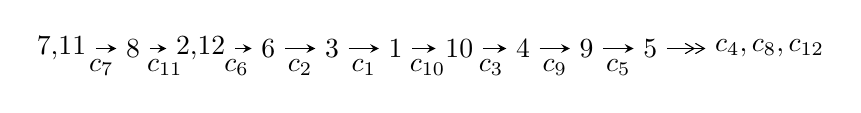
\begin{tikzpicture}[x=23pt, y=7pt]
	% node
	\node (A0) at (-1/8, 0) {7,11};
	\node (A1) at (1, 0) {8};
	\node (A2) at (33/16, 0) {2,12};
	\node (A3) at (25/8, 0) {6};
	\node (A4) at (33/8, 0) {3};
	\node (A5) at (41/8, 0) {1};
	\node (A6) at (49/8, 0) {10};
	\node (A7) at (57/8, 0) {4};
	\node (A8) at (65/8, 0) {9};
	\node (A9) at (73/8, 0) {5};
	\node (C1) at (1/2, -1) {$c_{7}$};
	\node (C2) at (3/2, -1) {$c_{11}$};
	\node (C3) at (21/8, -1) {$c_{6}$};
	\node (C4) at (29/8, -1) {$c_{2}$};
	\node (C5) at (37/8, -1) {$c_{1}$};
	\node (C6) at (45/8, -1) {$c_{10}$};
	\node (C7) at (53/8, -1) {$c_{3}$};
	\node (C8) at (61/8, -1) {$c_{9}$};
	\node (C9) at (69/8, -1) {$c_{5}$};
	\node (A10) at (11, 0) {$c_{4},c_{8},c_{12}$};

	% edge
	\draw[->,>=stealth]	
	(A0) edge (A1) (A1) edge (A2) (A2) edge (A3) (A3) edge (A4) (A4) edge (A5) (A5) edge (A6) (A6) edge (A7) (A7) edge (A8) (A8) edge (A9) ;
	\draw[->>,>={angle 60}]	
	(A9) edge (A10);
\end{tikzpicture} \\ 

\end{tabular} \\

\footnotetext{
The image of knot diagram is generated by the software ``\textbf{Draw programme}" developed by Andrew Bartholomew(\url{http://www.layer8.co.uk/maths/draw/index.htm\#Running-draw}), where we modified some parts for our purpose(\url{https://github.com/CATsTAILs/LinksPainter}).
}\phantom \\ \newline 
\centering \textbf{Ideals for irreducible components\footnotemark of $X_{\text{par}}$} 
 
\begin{align*}
I^u_{1}&=\langle 
b- u,\;-111497 u^{26}+189910 u^{25}+\cdots+191887 a-257923,\;u^{27}- u^{26}+\cdots+3 u-1\rangle \\
I^u_{2}&=\langle 
-5.40927\times10^{221} u^{103}-1.66221\times10^{222} u^{102}+\cdots+5.33227\times10^{221} b-3.81465\times10^{223},\\
\phantom{I^u_{2}}&\phantom{= \langle  }-3.26612\times10^{223} u^{103}-1.05210\times10^{224} u^{102}+\cdots+6.45205\times10^{223} a-7.33788\times10^{224},\\
\phantom{I^u_{2}}&\phantom{= \langle  }u^{104}+2 u^{103}+\cdots-17 u+121\rangle \\
I^u_{3}&=\langle 
b+u,\;2 u^{12}-2 u^{11}+6 u^{10}-5 u^9+12 u^8-9 u^7+13 u^6-8 u^5+8 u^4-5 u^3- u^2+a+u-1,\\
\phantom{I^u_{3}}&\phantom{= \langle  }u^{13}- u^{12}+4 u^{11}-3 u^{10}+9 u^9-6 u^8+13 u^7-7 u^6+12 u^5-6 u^4+6 u^3-3 u^2+u-1\rangle \\
I^u_{4}&=\langle 
- u^{13}+u^{12}-4 u^{11}+3 u^{10}-8 u^9+6 u^8-10 u^7+7 u^6-10 u^5+6 u^4-8 u^3+3 u^2+b-4 u+1,\\
\phantom{I^u_{4}}&\phantom{= \langle  }3 u^{12}-3 u^{11}+10 u^{10}-8 u^9+18 u^8-15 u^7+19 u^6-14 u^5+19 u^4-10 u^3+12 u^2+a-5 u+4,\\
\phantom{I^u_{4}}&\phantom{= \langle  }u^{14}- u^{13}+4 u^{12}-3 u^{11}+8 u^{10}-6 u^9+10 u^8-7 u^7+10 u^6-6 u^5+8 u^4-3 u^3+4 u^2- u+1\rangle \\
\\
\end{align*}
\raggedright * 4 irreducible components of $\dim_{\mathbb{C}}=0$, with total 158 representations.\\
\footnotetext{All coefficients of polynomials are rational numbers. But the coefficients are sometimes approximated in decimal forms when there is not enough margin.}
\newpage
\renewcommand{\arraystretch}{1}
\centering \section*{I. $I^u_{1}= \langle b- u,\;-1.11\times10^{5} u^{26}+1.90\times10^{5} u^{25}+\cdots+1.92\times10^{5} a-2.58\times10^{5},\;u^{27}- u^{26}+\cdots+3 u-1 \rangle$}
\flushleft \textbf{(i) Arc colorings}\\
\begin{tabular}{m{7pt} m{180pt} m{7pt} m{180pt} }
\flushright $a_{7}=$&$\begin{pmatrix}1\\0\end{pmatrix}$ \\
\flushright $a_{11}=$&$\begin{pmatrix}0\\u\end{pmatrix}$ \\
\flushright $a_{8}=$&$\begin{pmatrix}1\\- u^2\end{pmatrix}$ \\
\flushright $a_{2}=$&$\begin{pmatrix}0.581056 u^{26}-0.989697 u^{25}+\cdots+1.16938 u+1.34414\\u\end{pmatrix}$ \\
\flushright $a_{12}=$&$\begin{pmatrix}u\\u\end{pmatrix}$ \\
\flushright $a_{6}=$&$\begin{pmatrix}-0.408642 u^{26}-0.985012 u^{25}+\cdots-0.399027 u+1.58106\\u^2\end{pmatrix}$ \\
\flushright $a_{3}=$&$\begin{pmatrix}-0.812598 u^{26}+0.389719 u^{25}+\cdots+3.97636 u+0.935498\\u^3+u\end{pmatrix}$ \\
\flushright $a_{1}=$&$\begin{pmatrix}0.423645 u^{26}-0.450249 u^{25}+\cdots+1.62541 u+0.921261\\u^5+u^3+u\end{pmatrix}$ \\
\flushright $a_{10}=$&$\begin{pmatrix}u^3\\u^3+u\end{pmatrix}$ \\
\flushright $a_{4}=$&$\begin{pmatrix}-0.920328 u^{26}+0.782815 u^{25}+\cdots+4.86559 u+0.300943\\-1.12217 u^{26}+0.772976 u^{25}+\cdots+2.73671 u-0.593714\end{pmatrix}$ \\
\flushright $a_{9}=$&$\begin{pmatrix}-0.240814 u^{26}+0.615836 u^{25}+\cdots+1.05933 u-1.48438\\-0.245436 u^{26}+0.0573358 u^{25}+\cdots+1.36645 u-0.289717\end{pmatrix}$ \\
\flushright $a_{5}=$&$\begin{pmatrix}-0.462053 u^{26}+0.0205433 u^{25}+\cdots+2.63666 u+1.03217\\-0.245436 u^{26}+0.0573358 u^{25}+\cdots+1.36645 u-0.289717\end{pmatrix}$\\&\end{tabular}
\flushleft \textbf{(ii) Obstruction class $= -1$}\\~\\
\flushleft \textbf{(iii) Cusp Shapes $= \frac{922784}{191887} u^{26}-\frac{996775}{191887} u^{25}+\cdots-\frac{2303468}{191887} u+\frac{1548666}{191887}$}\\~\\
\newpage\renewcommand{\arraystretch}{1}
\flushleft \textbf{(iv) u-Polynomials at the component}\newline \\
\begin{tabular}{m{50pt}|m{274pt}}
Crossings & \hspace{64pt}u-Polynomials at each crossing \\
\hline $$\begin{aligned}c_{1},c_{10}\end{aligned}$$&$\begin{aligned}
&u^{27}+13 u^{26}+\cdots+3 u-1
\end{aligned}$\\
\hline $$\begin{aligned}c_{2},c_{6},c_{7}\\c_{11}\end{aligned}$$&$\begin{aligned}
&u^{27}- u^{26}+\cdots+3 u-1
\end{aligned}$\\
\hline $$\begin{aligned}c_{3}\end{aligned}$$&$\begin{aligned}
&u^{27}-22 u^{26}+\cdots+24576 u-2560
\end{aligned}$\\
\hline $$\begin{aligned}c_{4},c_{5},c_{8}\end{aligned}$$&$\begin{aligned}
&u^{27}+12 u^{26}+\cdots+16 u-32
\end{aligned}$\\
\hline $$\begin{aligned}c_{9},c_{12}\end{aligned}$$&$\begin{aligned}
&u^{27}- u^{26}+\cdots-3 u-1
\end{aligned}$\\
\hline
\end{tabular}\\~\\
\newpage\renewcommand{\arraystretch}{1}
\flushleft \textbf{(v) Riley Polynomials at the component}\newline \\
\begin{tabular}{m{50pt}|m{274pt}}
Crossings & \hspace{64pt}Riley Polynomials at each crossing \\
\hline $$\begin{aligned}c_{1},c_{10}\end{aligned}$$&$\begin{aligned}
&y^{27}+5 y^{26}+\cdots+87 y-1
\end{aligned}$\\
\hline $$\begin{aligned}c_{2},c_{6},c_{7}\\c_{11}\end{aligned}$$&$\begin{aligned}
&y^{27}+13 y^{26}+\cdots+3 y-1
\end{aligned}$\\
\hline $$\begin{aligned}c_{3}\end{aligned}$$&$\begin{aligned}
&y^{27}-6 y^{26}+\cdots-262144 y-6553600
\end{aligned}$\\
\hline $$\begin{aligned}c_{4},c_{5},c_{8}\end{aligned}$$&$\begin{aligned}
&y^{27}-24 y^{26}+\cdots+12032 y-1024
\end{aligned}$\\
\hline $$\begin{aligned}c_{9},c_{12}\end{aligned}$$&$\begin{aligned}
&y^{27}+11 y^{26}+\cdots-5 y-1
\end{aligned}$\\
\hline
\end{tabular}\\~\\
\newpage\flushleft \textbf{(vi) Complex Volumes and Cusp Shapes}
$$\begin{array}{c|c|c}  
\text{Solutions to }I^u_{1}& \I (\text{vol} + \sqrt{-1}CS) & \text{Cusp shape}\\
 \hline 
\begin{aligned}
u &= -0.798209 + 0.530470 I \\
a &= \phantom{-}0.734106 + 0.052162 I \\
b &= -0.798209 + 0.530470 I\end{aligned}
 & \phantom{-}4.09001 + 3.06443 I & \phantom{-}6.85135 - 1.90892 I \\ \hline\begin{aligned}
u &= -0.798209 - 0.530470 I \\
a &= \phantom{-}0.734106 - 0.052162 I \\
b &= -0.798209 - 0.530470 I\end{aligned}
 & \phantom{-}4.09001 - 3.06443 I & \phantom{-}6.85135 + 1.90892 I \\ \hline\begin{aligned}
u &= -0.426161 + 0.952205 I \\
a &= \phantom{-}4.12175 + 1.75502 I \\
b &= -0.426161 + 0.952205 I\end{aligned}
 & -9.45283 - 3.29114 I & -3.58272 + 7.60756 I \\ \hline\begin{aligned}
u &= -0.426161 - 0.952205 I \\
a &= \phantom{-}4.12175 - 1.75502 I \\
b &= -0.426161 - 0.952205 I\end{aligned}
 & -9.45283 + 3.29114 I & -3.58272 - 7.60756 I \\ \hline\begin{aligned}
u &= \phantom{-}0.954879 + 0.448921 I \\
a &= -0.281262 + 0.163354 I \\
b &= \phantom{-}0.954879 + 0.448921 I\end{aligned}
 & -1.43373 - 6.86787 I & \phantom{-}2.22098 + 3.48109 I \\ \hline\begin{aligned}
u &= \phantom{-}0.954879 - 0.448921 I \\
a &= -0.281262 - 0.163354 I \\
b &= \phantom{-}0.954879 - 0.448921 I\end{aligned}
 & -1.43373 + 6.86787 I & \phantom{-}2.22098 - 3.48109 I \\ \hline\begin{aligned}
u &= \phantom{-}0.385727 + 1.023230 I \\
a &= -0.12490 + 3.10427 I \\
b &= \phantom{-}0.385727 + 1.023230 I\end{aligned}
 & -2.90362 + 4.50575 I & -7.37031 - 4.71426 I \\ \hline\begin{aligned}
u &= \phantom{-}0.385727 - 1.023230 I \\
a &= -0.12490 - 3.10427 I \\
b &= \phantom{-}0.385727 - 1.023230 I\end{aligned}
 & -2.90362 - 4.50575 I & -7.37031 + 4.71426 I \\ \hline\begin{aligned}
u &= -0.212212 + 1.078960 I \\
a &= \phantom{-}0.50612 + 2.28652 I \\
b &= -0.212212 + 1.078960 I\end{aligned}
 & -5.61409 - 0.39405 I & -7.57855 - 0.70200 I \\ \hline\begin{aligned}
u &= -0.212212 - 1.078960 I \\
a &= \phantom{-}0.50612 - 2.28652 I \\
b &= -0.212212 - 1.078960 I\end{aligned}
 & -5.61409 + 0.39405 I & -7.57855 + 0.70200 I\\
 \hline 
 \end{array}$$\newpage$$\begin{array}{c|c|c}  
\text{Solutions to }I^u_{1}& \I (\text{vol} + \sqrt{-1}CS) & \text{Cusp shape}\\
 \hline 
\begin{aligned}
u &= \phantom{-}0.582844 + 0.672430 I \\
a &= -1.96986 - 0.14069 I \\
b &= \phantom{-}0.582844 + 0.672430 I\end{aligned}
 & \phantom{-}2.10068 + 1.61837 I & \phantom{-}4.51956 - 4.09176 I \\ \hline\begin{aligned}
u &= \phantom{-}0.582844 - 0.672430 I \\
a &= -1.96986 + 0.14069 I \\
b &= \phantom{-}0.582844 - 0.672430 I\end{aligned}
 & \phantom{-}2.10068 - 1.61837 I & \phantom{-}4.51956 + 4.09176 I \\ \hline\begin{aligned}
u &= \phantom{-}0.580393 + 1.018610 I \\
a &= -2.37719 + 1.54830 I \\
b &= \phantom{-}0.580393 + 1.018610 I\end{aligned}
 & -0.15243 + 7.74596 I & -1.13140 - 8.56215 I \\ \hline\begin{aligned}
u &= \phantom{-}0.580393 - 1.018610 I \\
a &= -2.37719 - 1.54830 I \\
b &= \phantom{-}0.580393 - 1.018610 I\end{aligned}
 & -0.15243 - 7.74596 I & -1.13140 + 8.56215 I \\ \hline\begin{aligned}
u &= \phantom{-}0.156183 + 1.196450 I \\
a &= -1.03361 + 2.66772 I \\
b &= \phantom{-}0.156183 + 1.196450 I\end{aligned}
 & -13.26850 - 1.40447 I & -9.24996 + 0.64080 I \\ \hline\begin{aligned}
u &= \phantom{-}0.156183 - 1.196450 I \\
a &= -1.03361 - 2.66772 I \\
b &= \phantom{-}0.156183 - 1.196450 I\end{aligned}
 & -13.26850 + 1.40447 I & -9.24996 - 0.64080 I \\ \hline\begin{aligned}
u &= -0.486526 + 1.105720 I \\
a &= \phantom{-}0.71115 + 2.96516 I \\
b &= -0.486526 + 1.105720 I\end{aligned}
 & -7.98758 - 9.88572 I & -5.51020 + 9.99998 I \\ \hline\begin{aligned}
u &= -0.486526 - 1.105720 I \\
a &= \phantom{-}0.71115 - 2.96516 I \\
b &= -0.486526 - 1.105720 I\end{aligned}
 & -7.98758 + 9.88572 I & -5.51020 - 9.99998 I \\ \hline\begin{aligned}
u &= -0.698815 + 0.260905 I \\
a &= -0.249931 + 0.254046 I \\
b &= -0.698815 + 0.260905 I\end{aligned}
 & -3.08031 + 1.04158 I & \phantom{-}0.697827 + 0.089058 I \\ \hline\begin{aligned}
u &= -0.698815 - 0.260905 I \\
a &= -0.249931 - 0.254046 I \\
b &= -0.698815 - 0.260905 I\end{aligned}
 & -3.08031 - 1.04158 I & \phantom{-}0.697827 - 0.089058 I\\
 \hline 
 \end{array}$$\newpage$$\begin{array}{c|c|c}  
\text{Solutions to }I^u_{1}& \I (\text{vol} + \sqrt{-1}CS) & \text{Cusp shape}\\
 \hline 
\begin{aligned}
u &= -0.646787 + 1.102220 I \\
a &= \phantom{-}1.64707 + 1.85074 I \\
b &= -0.646787 + 1.102220 I\end{aligned}
 & \phantom{-}0.59333 - 14.04150 I & \phantom{-}0.79014 + 10.59403 I \\ \hline\begin{aligned}
u &= -0.646787 - 1.102220 I \\
a &= \phantom{-}1.64707 - 1.85074 I \\
b &= -0.646787 - 1.102220 I\end{aligned}
 & \phantom{-}0.59333 + 14.04150 I & \phantom{-}0.79014 - 10.59403 I \\ \hline\begin{aligned}
u &= \phantom{-}0.282967 + 0.645901 I \\
a &= \phantom{-}0.678786 + 0.641978 I \\
b &= \phantom{-}0.282967 + 0.645901 I\end{aligned}
 & -0.20845 + 1.57682 I & -2.21035 - 5.49069 I \\ \hline\begin{aligned}
u &= \phantom{-}0.282967 - 0.645901 I \\
a &= \phantom{-}0.678786 - 0.641978 I \\
b &= \phantom{-}0.282967 - 0.645901 I\end{aligned}
 & -0.20845 - 1.57682 I & -2.21035 + 5.49069 I \\ \hline\begin{aligned}
u &= \phantom{-}0.663935 + 1.182010 I \\
a &= -1.32463 + 2.15062 I \\
b &= \phantom{-}0.663935 + 1.182010 I\end{aligned}
 & -6.0186 + 18.7694 I & -2.19898 - 10.24193 I \\ \hline\begin{aligned}
u &= \phantom{-}0.663935 - 1.182010 I \\
a &= -1.32463 - 2.15062 I \\
b &= \phantom{-}0.663935 - 1.182010 I\end{aligned}
 & -6.0186 - 18.7694 I & -2.19898 + 10.24193 I \\ \hline\begin{aligned}
u &= \phantom{-}0.323566\phantom{ +0.000000I} \\
a &= \phantom{-}1.92480\phantom{ +0.000000I} \\
b &= \phantom{-}0.323566\phantom{ +0.000000I}\end{aligned}
 & \phantom{-}1.13556\phantom{ +0.000000I} & \phantom{-}9.50520\phantom{ +0.000000I}\\
 \hline 
 \end{array}$$\newpage\newpage\renewcommand{\arraystretch}{1}
\centering \section*{II. $I^u_{2}= \langle -5.41\times10^{221} u^{103}-1.66\times10^{222} u^{102}+\cdots+5.33\times10^{221} b-3.81\times10^{223},\;-3.27\times10^{223} u^{103}-1.05\times10^{224} u^{102}+\cdots+6.45\times10^{223} a-7.34\times10^{224},\;u^{104}+2 u^{103}+\cdots-17 u+121 \rangle$}
\flushleft \textbf{(i) Arc colorings}\\
\begin{tabular}{m{7pt} m{180pt} m{7pt} m{180pt} }
\flushright $a_{7}=$&$\begin{pmatrix}1\\0\end{pmatrix}$ \\
\flushright $a_{11}=$&$\begin{pmatrix}0\\u\end{pmatrix}$ \\
\flushright $a_{8}=$&$\begin{pmatrix}1\\- u^2\end{pmatrix}$ \\
\flushright $a_{2}=$&$\begin{pmatrix}0.506215 u^{103}+1.63064 u^{102}+\cdots+29.3200 u+11.3730\\1.01444 u^{103}+3.11726 u^{102}+\cdots+221.790 u+71.5390\end{pmatrix}$ \\
\flushright $a_{12}=$&$\begin{pmatrix}u\\u\end{pmatrix}$ \\
\flushright $a_{6}=$&$\begin{pmatrix}-1.01826 u^{103}-1.89566 u^{102}+\cdots-98.4955 u+153.705\\-0.962126 u^{103}-1.98060 u^{102}+\cdots-150.377 u+97.0479\end{pmatrix}$ \\
\flushright $a_{3}=$&$\begin{pmatrix}-0.104590 u^{103}-0.264231 u^{102}+\cdots-275.043 u-157.743\\0.835266 u^{103}+1.18555 u^{102}+\cdots-72.8082 u-246.443\end{pmatrix}$ \\
\flushright $a_{1}=$&$\begin{pmatrix}-0.758472 u^{103}-1.35795 u^{102}+\cdots-193.645 u+109.101\\0.136944 u^{103}+0.870777 u^{102}+\cdots-101.859 u+34.2650\end{pmatrix}$ \\
\flushright $a_{10}=$&$\begin{pmatrix}u^3\\u^3+u\end{pmatrix}$ \\
\flushright $a_{4}=$&$\begin{pmatrix}-0.0375614 u^{103}-0.896782 u^{102}+\cdots-369.104 u-256.644\\1.79450 u^{103}+3.15476 u^{102}+\cdots-75.5459 u-381.742\end{pmatrix}$ \\
\flushright $a_{9}=$&$\begin{pmatrix}-0.129934 u^{103}-0.0682942 u^{102}+\cdots+180.501 u+129.995\\0.351406 u^{103}+1.08238 u^{102}+\cdots+73.6035 u+75.0223\end{pmatrix}$ \\
\flushright $a_{5}=$&$\begin{pmatrix}-1.05156 u^{103}-1.82989 u^{102}+\cdots-284.135 u+25.6770\\0.0400246 u^{103}-0.880599 u^{102}+\cdots-216.852 u-249.262\end{pmatrix}$\\&\end{tabular}
\flushleft \textbf{(ii) Obstruction class $= -1$}\\~\\
\flushleft \textbf{(iii) Cusp Shapes $= 1.64573 u^{103}+4.55387 u^{102}+\cdots+785.939 u+299.162$}\\~\\
\newpage\renewcommand{\arraystretch}{1}
\flushleft \textbf{(iv) u-Polynomials at the component}\newline \\
\begin{tabular}{m{50pt}|m{274pt}}
Crossings & \hspace{64pt}u-Polynomials at each crossing \\
\hline $$\begin{aligned}c_{1},c_{10}\end{aligned}$$&$\begin{aligned}
&u^{104}+46 u^{103}+\cdots+249939 u+14641
\end{aligned}$\\
\hline $$\begin{aligned}c_{2},c_{6},c_{7}\\c_{11}\end{aligned}$$&$\begin{aligned}
&u^{104}+2 u^{103}+\cdots-17 u+121
\end{aligned}$\\
\hline $$\begin{aligned}c_{3}\end{aligned}$$&$\begin{aligned}
&(u^{52}+10 u^{51}+\cdots-3 u-1)^{2}
\end{aligned}$\\
\hline $$\begin{aligned}c_{4},c_{5},c_{8}\end{aligned}$$&$\begin{aligned}
&(u^{52}-5 u^{51}+\cdots+7 u+1)^{2}
\end{aligned}$\\
\hline $$\begin{aligned}c_{9},c_{12}\end{aligned}$$&$\begin{aligned}
&u^{104}+13 u^{103}+\cdots+3452 u+283
\end{aligned}$\\
\hline
\end{tabular}\\~\\
\newpage\renewcommand{\arraystretch}{1}
\flushleft \textbf{(v) Riley Polynomials at the component}\newline \\
\begin{tabular}{m{50pt}|m{274pt}}
Crossings & \hspace{64pt}Riley Polynomials at each crossing \\
\hline $$\begin{aligned}c_{1},c_{10}\end{aligned}$$&$\begin{aligned}
&y^{104}+34 y^{103}+\cdots+3659910927 y+214358881
\end{aligned}$\\
\hline $$\begin{aligned}c_{2},c_{6},c_{7}\\c_{11}\end{aligned}$$&$\begin{aligned}
&y^{104}+46 y^{103}+\cdots+249939 y+14641
\end{aligned}$\\
\hline $$\begin{aligned}c_{3}\end{aligned}$$&$\begin{aligned}
&(y^{52}-12 y^{51}+\cdots-43 y+1)^{2}
\end{aligned}$\\
\hline $$\begin{aligned}c_{4},c_{5},c_{8}\end{aligned}$$&$\begin{aligned}
&(y^{52}-53 y^{51}+\cdots-37 y+1)^{2}
\end{aligned}$\\
\hline $$\begin{aligned}c_{9},c_{12}\end{aligned}$$&$\begin{aligned}
&y^{104}-5 y^{103}+\cdots+215340 y+80089
\end{aligned}$\\
\hline
\end{tabular}\\~\\
\newpage\flushleft \textbf{(vi) Complex Volumes and Cusp Shapes}
$$\begin{array}{c|c|c}  
\text{Solutions to }I^u_{2}& \I (\text{vol} + \sqrt{-1}CS) & \text{Cusp shape}\\
 \hline 
\begin{aligned}
u &= -0.601006 + 0.783368 I \\
a &= \phantom{-}0.0584591 + 0.0734378 I \\
b &= \phantom{-}0.723694 + 1.004170 I\end{aligned}
 & \phantom{-}1.55323 + 1.66347 I & \phantom{-0.000000 } 0 \\ \hline\begin{aligned}
u &= -0.601006 - 0.783368 I \\
a &= \phantom{-}0.0584591 - 0.0734378 I \\
b &= \phantom{-}0.723694 - 1.004170 I\end{aligned}
 & \phantom{-}1.55323 - 1.66347 I & \phantom{-0.000000 } 0 \\ \hline\begin{aligned}
u &= -0.625964 + 0.763245 I \\
a &= \phantom{-}0.130359 - 0.723406 I \\
b &= \phantom{-}0.924850 + 0.421097 I\end{aligned}
 & \phantom{-}3.26376 - 0.55062 I & \phantom{-0.000000 } 0 \\ \hline\begin{aligned}
u &= -0.625964 - 0.763245 I \\
a &= \phantom{-}0.130359 + 0.723406 I \\
b &= \phantom{-}0.924850 - 0.421097 I\end{aligned}
 & \phantom{-}3.26376 + 0.55062 I & \phantom{-0.000000 } 0 \\ \hline\begin{aligned}
u &= \phantom{-}0.924850 + 0.421097 I \\
a &= \phantom{-}0.646631 + 0.302782 I \\
b &= -0.625964 + 0.763245 I\end{aligned}
 & \phantom{-}3.26376 - 0.55062 I & \phantom{-0.000000 } 0 \\ \hline\begin{aligned}
u &= \phantom{-}0.924850 - 0.421097 I \\
a &= \phantom{-}0.646631 - 0.302782 I \\
b &= -0.625964 - 0.763245 I\end{aligned}
 & \phantom{-}3.26376 + 0.55062 I & \phantom{-0.000000 } 0 \\ \hline\begin{aligned}
u &= \phantom{-}0.031250 + 0.980911 I \\
a &= -0.235677 + 0.376852 I \\
b &= -0.635597 + 0.291200 I\end{aligned}
 & -1.55506 + 2.06501 I & \phantom{-0.000000 } 0 \\ \hline\begin{aligned}
u &= \phantom{-}0.031250 - 0.980911 I \\
a &= -0.235677 - 0.376852 I \\
b &= -0.635597 - 0.291200 I\end{aligned}
 & -1.55506 - 2.06501 I & \phantom{-0.000000 } 0 \\ \hline\begin{aligned}
u &= -0.851961 + 0.480235 I \\
a &= \phantom{-}0.859609 - 0.480965 I \\
b &= -0.641480 - 1.066260 I\end{aligned}
 & \phantom{-}2.47458 + 8.47773 I & \phantom{-0.000000 } 0 \\ \hline\begin{aligned}
u &= -0.851961 - 0.480235 I \\
a &= \phantom{-}0.859609 + 0.480965 I \\
b &= -0.641480 + 1.066260 I\end{aligned}
 & \phantom{-}2.47458 - 8.47773 I & \phantom{-0.000000 } 0\\
 \hline 
 \end{array}$$\newpage$$\begin{array}{c|c|c}  
\text{Solutions to }I^u_{2}& \I (\text{vol} + \sqrt{-1}CS) & \text{Cusp shape}\\
 \hline 
\begin{aligned}
u &= -1.029580 + 0.075923 I \\
a &= -0.916980 + 1.015670 I \\
b &= \phantom{-}0.480542 + 0.932970 I\end{aligned}
 & -1.46501 + 2.48222 I & \phantom{-0.000000 } 0 \\ \hline\begin{aligned}
u &= -1.029580 - 0.075923 I \\
a &= -0.916980 - 1.015670 I \\
b &= \phantom{-}0.480542 - 0.932970 I\end{aligned}
 & -1.46501 - 2.48222 I & \phantom{-0.000000 } 0 \\ \hline\begin{aligned}
u &= \phantom{-}0.295716 + 0.919872 I \\
a &= -0.32064 - 2.78318 I \\
b &= \phantom{-}0.487555 - 1.059280 I\end{aligned}
 & -2.18861 - 2.12521 I & \phantom{-0.000000 } 0 \\ \hline\begin{aligned}
u &= \phantom{-}0.295716 - 0.919872 I \\
a &= -0.32064 + 2.78318 I \\
b &= \phantom{-}0.487555 + 1.059280 I\end{aligned}
 & -2.18861 + 2.12521 I & \phantom{-0.000000 } 0 \\ \hline\begin{aligned}
u &= \phantom{-}0.425973 + 0.861359 I \\
a &= \phantom{-}0.528034 + 0.144800 I \\
b &= \phantom{-}0.441668 + 0.214876 I\end{aligned}
 & -0.11368 + 1.81640 I & \phantom{-0.000000 } 0 \\ \hline\begin{aligned}
u &= \phantom{-}0.425973 - 0.861359 I \\
a &= \phantom{-}0.528034 - 0.144800 I \\
b &= \phantom{-}0.441668 - 0.214876 I\end{aligned}
 & -0.11368 - 1.81640 I & \phantom{-0.000000 } 0 \\ \hline\begin{aligned}
u &= \phantom{-}0.480542 + 0.932970 I \\
a &= -0.566525 - 1.221080 I \\
b &= -1.029580 + 0.075923 I\end{aligned}
 & -1.46501 + 2.48222 I & \phantom{-0.000000 } 0 \\ \hline\begin{aligned}
u &= \phantom{-}0.480542 - 0.932970 I \\
a &= -0.566525 + 1.221080 I \\
b &= -1.029580 - 0.075923 I\end{aligned}
 & -1.46501 - 2.48222 I & \phantom{-0.000000 } 0 \\ \hline\begin{aligned}
u &= \phantom{-}0.429770 + 0.968741 I \\
a &= -1.21282 + 1.70756 I \\
b &= -0.546527 + 1.284080 I\end{aligned}
 & -5.52629 - 2.94682 I & \phantom{-0.000000 } 0 \\ \hline\begin{aligned}
u &= \phantom{-}0.429770 - 0.968741 I \\
a &= -1.21282 - 1.70756 I \\
b &= -0.546527 - 1.284080 I\end{aligned}
 & -5.52629 + 2.94682 I & \phantom{-0.000000 } 0\\
 \hline 
 \end{array}$$\newpage$$\begin{array}{c|c|c}  
\text{Solutions to }I^u_{2}& \I (\text{vol} + \sqrt{-1}CS) & \text{Cusp shape}\\
 \hline 
\begin{aligned}
u &= \phantom{-}0.986696 + 0.396692 I \\
a &= -0.624859 - 0.884889 I \\
b &= \phantom{-}0.672647 - 1.153190 I\end{aligned}
 & -3.60087 - 12.79700 I & \phantom{-0.000000 } 0 \\ \hline\begin{aligned}
u &= \phantom{-}0.986696 - 0.396692 I \\
a &= -0.624859 + 0.884889 I \\
b &= \phantom{-}0.672647 + 1.153190 I\end{aligned}
 & -3.60087 + 12.79700 I & \phantom{-0.000000 } 0 \\ \hline\begin{aligned}
u &= -0.922258 + 0.122473 I \\
a &= -0.424499 + 0.044620 I \\
b &= \phantom{-}0.438182 - 0.776661 I\end{aligned}
 & -0.90908 - 1.34820 I & \phantom{-0.000000 } 0 \\ \hline\begin{aligned}
u &= -0.922258 - 0.122473 I \\
a &= -0.424499 - 0.044620 I \\
b &= \phantom{-}0.438182 + 0.776661 I\end{aligned}
 & -0.90908 + 1.34820 I & \phantom{-0.000000 } 0 \\ \hline\begin{aligned}
u &= \phantom{-}0.902428 + 0.580570 I \\
a &= \phantom{-}0.944671 - 0.522436 I \\
b &= -0.606198 - 0.907558 I\end{aligned}
 & \phantom{-}2.81324 + 4.29790 I & \phantom{-0.000000 } 0 \\ \hline\begin{aligned}
u &= \phantom{-}0.902428 - 0.580570 I \\
a &= \phantom{-}0.944671 + 0.522436 I \\
b &= -0.606198 + 0.907558 I\end{aligned}
 & \phantom{-}2.81324 - 4.29790 I & \phantom{-0.000000 } 0 \\ \hline\begin{aligned}
u &= \phantom{-}0.776726 + 0.758218 I \\
a &= -0.363743 - 0.173713 I \\
b &= -1.103830 + 0.728123 I\end{aligned}
 & -0.184790 - 0.909141 I & \phantom{-0.000000 } 0 \\ \hline\begin{aligned}
u &= \phantom{-}0.776726 - 0.758218 I \\
a &= -0.363743 + 0.173713 I \\
b &= -1.103830 - 0.728123 I\end{aligned}
 & -0.184790 + 0.909141 I & \phantom{-0.000000 } 0 \\ \hline\begin{aligned}
u &= -0.606198 + 0.907558 I \\
a &= -0.646877 - 0.841459 I \\
b &= \phantom{-}0.902428 - 0.580570 I\end{aligned}
 & \phantom{-}2.81324 - 4.29790 I & \phantom{-0.000000 } 0 \\ \hline\begin{aligned}
u &= -0.606198 - 0.907558 I \\
a &= -0.646877 + 0.841459 I \\
b &= \phantom{-}0.902428 + 0.580570 I\end{aligned}
 & \phantom{-}2.81324 + 4.29790 I & \phantom{-0.000000 } 0\\
 \hline 
 \end{array}$$\newpage$$\begin{array}{c|c|c}  
\text{Solutions to }I^u_{2}& \I (\text{vol} + \sqrt{-1}CS) & \text{Cusp shape}\\
 \hline 
\begin{aligned}
u &= \phantom{-}0.499516 + 0.974559 I \\
a &= \phantom{-}1.75948 - 2.30223 I \\
b &= -0.64443 - 1.29302 I\end{aligned}
 & -5.06786 + 8.46879 I & \phantom{-0.000000 } 0 \\ \hline\begin{aligned}
u &= \phantom{-}0.499516 - 0.974559 I \\
a &= \phantom{-}1.75948 + 2.30223 I \\
b &= -0.64443 + 1.29302 I\end{aligned}
 & -5.06786 - 8.46879 I & \phantom{-0.000000 } 0 \\ \hline\begin{aligned}
u &= -0.633873 + 0.899833 I \\
a &= -1.40684 - 1.55880 I \\
b &= \phantom{-}0.710426 - 1.119870 I\end{aligned}
 & \phantom{-}1.20873 - 6.54051 I & \phantom{-0.000000 } 0 \\ \hline\begin{aligned}
u &= -0.633873 - 0.899833 I \\
a &= -1.40684 + 1.55880 I \\
b &= \phantom{-}0.710426 + 1.119870 I\end{aligned}
 & \phantom{-}1.20873 + 6.54051 I & \phantom{-0.000000 } 0 \\ \hline\begin{aligned}
u &= \phantom{-}0.438182 + 0.776661 I \\
a &= \phantom{-}0.303685 - 0.325708 I \\
b &= -0.922258 - 0.122473 I\end{aligned}
 & -0.90908 + 1.34820 I & \phantom{-0.000000 } 0 \\ \hline\begin{aligned}
u &= \phantom{-}0.438182 - 0.776661 I \\
a &= \phantom{-}0.303685 + 0.325708 I \\
b &= -0.922258 + 0.122473 I\end{aligned}
 & -0.90908 - 1.34820 I & \phantom{-0.000000 } 0 \\ \hline\begin{aligned}
u &= -0.354334 + 0.817967 I \\
a &= \phantom{-}1.38616 + 3.19989 I \\
b &= -0.354334 - 0.817967 I\end{aligned}
 & -8.87842\phantom{ +0.000000I} & \phantom{-0.000000 } 0 \\ \hline\begin{aligned}
u &= -0.354334 - 0.817967 I \\
a &= \phantom{-}1.38616 - 3.19989 I \\
b &= -0.354334 + 0.817967 I\end{aligned}
 & -8.87842\phantom{ +0.000000I} & \phantom{-0.000000 } 0 \\ \hline\begin{aligned}
u &= \phantom{-}0.785536 + 0.418604 I \\
a &= -0.544261 + 1.279960 I \\
b &= \phantom{-}0.008149 + 1.329420 I\end{aligned}
 & -8.10565 - 3.93282 I & \phantom{-0.000000 } 0 \\ \hline\begin{aligned}
u &= \phantom{-}0.785536 - 0.418604 I \\
a &= -0.544261 - 1.279960 I \\
b &= \phantom{-}0.008149 - 1.329420 I\end{aligned}
 & -8.10565 + 3.93282 I & \phantom{-0.000000 } 0\\
 \hline 
 \end{array}$$\newpage$$\begin{array}{c|c|c}  
\text{Solutions to }I^u_{2}& \I (\text{vol} + \sqrt{-1}CS) & \text{Cusp shape}\\
 \hline 
\begin{aligned}
u &= \phantom{-}0.558791 + 0.968003 I \\
a &= -0.063595 + 1.107100 I \\
b &= \phantom{-}0.641644 - 0.575513 I\end{aligned}
 & \phantom{-}1.18258 + 2.94175 I & \phantom{-0.000000 } 0 \\ \hline\begin{aligned}
u &= \phantom{-}0.558791 - 0.968003 I \\
a &= -0.063595 - 1.107100 I \\
b &= \phantom{-}0.641644 + 0.575513 I\end{aligned}
 & \phantom{-}1.18258 - 2.94175 I & \phantom{-0.000000 } 0 \\ \hline\begin{aligned}
u &= -0.504260 + 1.007480 I \\
a &= -0.41215 - 2.73765 I \\
b &= -0.366905 - 1.121840 I\end{aligned}
 & -8.78594 - 2.32359 I & \phantom{-0.000000 } 0 \\ \hline\begin{aligned}
u &= -0.504260 - 1.007480 I \\
a &= -0.41215 + 2.73765 I \\
b &= -0.366905 + 1.121840 I\end{aligned}
 & -8.78594 + 2.32359 I & \phantom{-0.000000 } 0 \\ \hline\begin{aligned}
u &= \phantom{-}0.641644 + 0.575513 I \\
a &= -1.38782 + 0.37658 I \\
b &= \phantom{-}0.558791 - 0.968003 I\end{aligned}
 & \phantom{-}1.18258 - 2.94175 I & \phantom{-0.000000 } 0 \\ \hline\begin{aligned}
u &= \phantom{-}0.641644 - 0.575513 I \\
a &= -1.38782 - 0.37658 I \\
b &= \phantom{-}0.558791 + 0.968003 I\end{aligned}
 & \phantom{-}1.18258 + 2.94175 I & \phantom{-0.000000 } 0 \\ \hline\begin{aligned}
u &= \phantom{-}0.487555 + 1.059280 I \\
a &= \phantom{-}1.75487 - 1.51966 I \\
b &= \phantom{-}0.295716 - 0.919872 I\end{aligned}
 & -2.18861 + 2.12521 I & \phantom{-0.000000 } 0 \\ \hline\begin{aligned}
u &= \phantom{-}0.487555 - 1.059280 I \\
a &= \phantom{-}1.75487 + 1.51966 I \\
b &= \phantom{-}0.295716 + 0.919872 I\end{aligned}
 & -2.18861 - 2.12521 I & \phantom{-0.000000 } 0 \\ \hline\begin{aligned}
u &= -0.252289 + 1.144220 I \\
a &= -0.90905 + 1.41665 I \\
b &= -0.547375 + 0.522103 I\end{aligned}
 & -7.35313 - 1.89826 I & \phantom{-0.000000 } 0 \\ \hline\begin{aligned}
u &= -0.252289 - 1.144220 I \\
a &= -0.90905 - 1.41665 I \\
b &= -0.547375 - 0.522103 I\end{aligned}
 & -7.35313 + 1.89826 I & \phantom{-0.000000 } 0\\
 \hline 
 \end{array}$$\newpage$$\begin{array}{c|c|c}  
\text{Solutions to }I^u_{2}& \I (\text{vol} + \sqrt{-1}CS) & \text{Cusp shape}\\
 \hline 
\begin{aligned}
u &= \phantom{-}0.442489 + 0.697558 I \\
a &= -0.0215440 + 0.0999968 I \\
b &= -0.673127 + 1.235190 I\end{aligned}
 & -4.12299 - 4.50302 I & \phantom{-0.000000 } 0 \\ \hline\begin{aligned}
u &= \phantom{-}0.442489 - 0.697558 I \\
a &= -0.0215440 - 0.0999968 I \\
b &= -0.673127 - 1.235190 I\end{aligned}
 & -4.12299 + 4.50302 I & \phantom{-0.000000 } 0 \\ \hline\begin{aligned}
u &= -0.366905 + 1.121840 I \\
a &= -1.55841 - 2.13414 I \\
b &= -0.504260 - 1.007480 I\end{aligned}
 & -8.78594 + 2.32359 I & \phantom{-0.000000 } 0 \\ \hline\begin{aligned}
u &= -0.366905 - 1.121840 I \\
a &= -1.55841 + 2.13414 I \\
b &= -0.504260 + 1.007480 I\end{aligned}
 & -8.78594 - 2.32359 I & \phantom{-0.000000 } 0 \\ \hline\begin{aligned}
u &= \phantom{-}0.037861 + 1.180360 I \\
a &= \phantom{-}0.16520 - 1.99220 I \\
b &= -0.536637 - 1.062390 I\end{aligned}
 & -3.63796 + 6.54304 I & \phantom{-0.000000 } 0 \\ \hline\begin{aligned}
u &= \phantom{-}0.037861 - 1.180360 I \\
a &= \phantom{-}0.16520 + 1.99220 I \\
b &= -0.536637 + 1.062390 I\end{aligned}
 & -3.63796 - 6.54304 I & \phantom{-0.000000 } 0 \\ \hline\begin{aligned}
u &= -0.536637 + 1.062390 I \\
a &= -0.98281 - 1.72288 I \\
b &= \phantom{-}0.037861 - 1.180360 I\end{aligned}
 & -3.63796 - 6.54304 I & \phantom{-0.000000 } 0 \\ \hline\begin{aligned}
u &= -0.536637 - 1.062390 I \\
a &= -0.98281 + 1.72288 I \\
b &= \phantom{-}0.037861 + 1.180360 I\end{aligned}
 & -3.63796 + 6.54304 I & \phantom{-0.000000 } 0 \\ \hline\begin{aligned}
u &= \phantom{-}0.724416 + 0.947735 I \\
a &= \phantom{-}0.52725 - 1.41910 I \\
b &= -1.058660 - 0.927148 I\end{aligned}
 & -0.76003 + 6.57704 I & \phantom{-0.000000 } 0 \\ \hline\begin{aligned}
u &= \phantom{-}0.724416 - 0.947735 I \\
a &= \phantom{-}0.52725 + 1.41910 I \\
b &= -1.058660 + 0.927148 I\end{aligned}
 & -0.76003 - 6.57704 I & \phantom{-0.000000 } 0\\
 \hline 
 \end{array}$$\newpage$$\begin{array}{c|c|c}  
\text{Solutions to }I^u_{2}& \I (\text{vol} + \sqrt{-1}CS) & \text{Cusp shape}\\
 \hline 
\begin{aligned}
u &= \phantom{-}0.409809 + 1.125960 I \\
a &= \phantom{-}0.05894 + 1.41666 I \\
b &= -0.217013 + 0.721229 I\end{aligned}
 & -1.44654 + 2.79038 I & \phantom{-0.000000 } 0 \\ \hline\begin{aligned}
u &= \phantom{-}0.409809 - 1.125960 I \\
a &= \phantom{-}0.05894 - 1.41666 I \\
b &= -0.217013 - 0.721229 I\end{aligned}
 & -1.44654 - 2.79038 I & \phantom{-0.000000 } 0 \\ \hline\begin{aligned}
u &= -0.543575 + 1.094100 I \\
a &= -0.769980 + 0.146024 I \\
b &= -0.598812 - 0.128338 I\end{aligned}
 & -5.39609 - 5.71097 I & \phantom{-0.000000 } 0 \\ \hline\begin{aligned}
u &= -0.543575 - 1.094100 I \\
a &= -0.769980 - 0.146024 I \\
b &= -0.598812 + 0.128338 I\end{aligned}
 & -5.39609 + 5.71097 I & \phantom{-0.000000 } 0 \\ \hline\begin{aligned}
u &= \phantom{-}0.723694 + 1.004170 I \\
a &= -0.0426830 + 0.0615170 I \\
b &= -0.601006 + 0.783368 I\end{aligned}
 & \phantom{-}1.55323 + 1.66347 I & \phantom{-0.000000 } 0 \\ \hline\begin{aligned}
u &= \phantom{-}0.723694 - 1.004170 I \\
a &= -0.0426830 - 0.0615170 I \\
b &= -0.601006 - 0.783368 I\end{aligned}
 & \phantom{-}1.55323 - 1.66347 I & \phantom{-0.000000 } 0 \\ \hline\begin{aligned}
u &= -0.547375 + 0.522103 I \\
a &= \phantom{-}0.05604 + 2.60664 I \\
b &= -0.252289 + 1.144220 I\end{aligned}
 & -7.35313 - 1.89826 I & -3.11574 + 3.33363 I \\ \hline\begin{aligned}
u &= -0.547375 - 0.522103 I \\
a &= \phantom{-}0.05604 - 2.60664 I \\
b &= -0.252289 - 1.144220 I\end{aligned}
 & -7.35313 + 1.89826 I & -3.11574 - 3.33363 I \\ \hline\begin{aligned}
u &= -0.641480 + 1.066260 I \\
a &= -0.358729 + 0.686039 I \\
b &= -0.851961 - 0.480235 I\end{aligned}
 & \phantom{-}2.47458 - 8.47773 I & \phantom{-0.000000 } 0 \\ \hline\begin{aligned}
u &= -0.641480 - 1.066260 I \\
a &= -0.358729 - 0.686039 I \\
b &= -0.851961 + 0.480235 I\end{aligned}
 & \phantom{-}2.47458 + 8.47773 I & \phantom{-0.000000 } 0\\
 \hline 
 \end{array}$$\newpage$$\begin{array}{c|c|c}  
\text{Solutions to }I^u_{2}& \I (\text{vol} + \sqrt{-1}CS) & \text{Cusp shape}\\
 \hline 
\begin{aligned}
u &= -0.217013 + 0.721229 I \\
a &= \phantom{-}1.42348 + 1.74983 I \\
b &= \phantom{-}0.409809 + 1.125960 I\end{aligned}
 & -1.44654 + 2.79038 I & -3.18108 - 7.81868 I \\ \hline\begin{aligned}
u &= -0.217013 - 0.721229 I \\
a &= \phantom{-}1.42348 - 1.74983 I \\
b &= \phantom{-}0.409809 - 1.125960 I\end{aligned}
 & -1.44654 - 2.79038 I & -3.18108 + 7.81868 I \\ \hline\begin{aligned}
u &= \phantom{-}0.269989 + 0.699887 I \\
a &= \phantom{-}0.79505 - 1.96652 I \\
b &= -0.531628 - 1.197670 I\end{aligned}
 & -4.54291 + 6.20206 I & -3.22343 - 7.94187 I \\ \hline\begin{aligned}
u &= \phantom{-}0.269989 - 0.699887 I \\
a &= \phantom{-}0.79505 + 1.96652 I \\
b &= -0.531628 + 1.197670 I\end{aligned}
 & -4.54291 - 6.20206 I & -3.22343 + 7.94187 I \\ \hline\begin{aligned}
u &= \phantom{-}0.617899 + 1.107080 I \\
a &= \phantom{-}1.03560 - 1.95299 I \\
b &= \phantom{-}0.079207 - 1.395880 I\end{aligned}
 & -10.12590 + 9.22402 I & \phantom{-0.000000 } 0 \\ \hline\begin{aligned}
u &= \phantom{-}0.617899 - 1.107080 I \\
a &= \phantom{-}1.03560 + 1.95299 I \\
b &= \phantom{-}0.079207 + 1.395880 I\end{aligned}
 & -10.12590 - 9.22402 I & \phantom{-0.000000 } 0 \\ \hline\begin{aligned}
u &= \phantom{-}0.223884 + 0.677776 I \\
a &= \phantom{-}1.02403 - 3.10009 I \\
b &= \phantom{-}0.223884 - 0.677776 I\end{aligned}
 & \phantom{-}0.423251\phantom{ +0.000000I} & -1.45472 + 0. I\phantom{ +0.000000I} \\ \hline\begin{aligned}
u &= \phantom{-}0.223884 - 0.677776 I \\
a &= \phantom{-}1.02403 + 3.10009 I \\
b &= \phantom{-}0.223884 + 0.677776 I\end{aligned}
 & \phantom{-}0.423251\phantom{ +0.000000I} & -1.45472 + 0. I\phantom{ +0.000000I} \\ \hline\begin{aligned}
u &= -0.635597 + 0.291200 I \\
a &= \phantom{-}0.359559 + 0.509922 I \\
b &= \phantom{-}0.031250 + 0.980911 I\end{aligned}
 & -1.55506 + 2.06501 I & -1.16113 - 4.48303 I \\ \hline\begin{aligned}
u &= -0.635597 - 0.291200 I \\
a &= \phantom{-}0.359559 - 0.509922 I \\
b &= \phantom{-}0.031250 - 0.980911 I\end{aligned}
 & -1.55506 - 2.06501 I & -1.16113 + 4.48303 I\\
 \hline 
 \end{array}$$\newpage$$\begin{array}{c|c|c}  
\text{Solutions to }I^u_{2}& \I (\text{vol} + \sqrt{-1}CS) & \text{Cusp shape}\\
 \hline 
\begin{aligned}
u &= -0.531628 + 1.197670 I \\
a &= -0.510395 - 1.101850 I \\
b &= \phantom{-}0.269989 - 0.699887 I\end{aligned}
 & -4.54291 - 6.20206 I & \phantom{-0.000000 } 0 \\ \hline\begin{aligned}
u &= -0.531628 - 1.197670 I \\
a &= -0.510395 + 1.101850 I \\
b &= \phantom{-}0.269989 + 0.699887 I\end{aligned}
 & -4.54291 + 6.20206 I & \phantom{-0.000000 } 0 \\ \hline\begin{aligned}
u &= -1.103830 + 0.728123 I \\
a &= -0.075822 + 0.322076 I \\
b &= \phantom{-}0.776726 + 0.758218 I\end{aligned}
 & -0.184790 - 0.909141 I & \phantom{-0.000000 } 0 \\ \hline\begin{aligned}
u &= -1.103830 - 0.728123 I \\
a &= -0.075822 - 0.322076 I \\
b &= \phantom{-}0.776726 - 0.758218 I\end{aligned}
 & -0.184790 + 0.909141 I & \phantom{-0.000000 } 0 \\ \hline\begin{aligned}
u &= \phantom{-}0.710426 + 1.119870 I \\
a &= \phantom{-}1.10367 - 1.34867 I \\
b &= -0.633873 - 0.899833 I\end{aligned}
 & \phantom{-}1.20873 + 6.54051 I & \phantom{-0.000000 } 0 \\ \hline\begin{aligned}
u &= \phantom{-}0.710426 - 1.119870 I \\
a &= \phantom{-}1.10367 + 1.34867 I \\
b &= -0.633873 + 0.899833 I\end{aligned}
 & \phantom{-}1.20873 - 6.54051 I & \phantom{-0.000000 } 0 \\ \hline\begin{aligned}
u &= \phantom{-}0.008149 + 1.329420 I \\
a &= \phantom{-}0.580472 + 0.728186 I \\
b &= \phantom{-}0.785536 + 0.418604 I\end{aligned}
 & -8.10565 - 3.93282 I & \phantom{-0.000000 } 0 \\ \hline\begin{aligned}
u &= \phantom{-}0.008149 - 1.329420 I \\
a &= \phantom{-}0.580472 - 0.728186 I \\
b &= \phantom{-}0.785536 - 0.418604 I\end{aligned}
 & -8.10565 + 3.93282 I & \phantom{-0.000000 } 0 \\ \hline\begin{aligned}
u &= \phantom{-}0.672647 + 1.153190 I \\
a &= \phantom{-}0.625101 + 0.594864 I \\
b &= \phantom{-}0.986696 - 0.396692 I\end{aligned}
 & -3.60087 + 12.79700 I & \phantom{-0.000000 } 0 \\ \hline\begin{aligned}
u &= \phantom{-}0.672647 - 1.153190 I \\
a &= \phantom{-}0.625101 - 0.594864 I \\
b &= \phantom{-}0.986696 + 0.396692 I\end{aligned}
 & -3.60087 - 12.79700 I & \phantom{-0.000000 } 0\\
 \hline 
 \end{array}$$\newpage$$\begin{array}{c|c|c}  
\text{Solutions to }I^u_{2}& \I (\text{vol} + \sqrt{-1}CS) & \text{Cusp shape}\\
 \hline 
\begin{aligned}
u &= -0.598812 + 0.128338 I \\
a &= -0.09774 - 1.56034 I \\
b &= -0.543575 - 1.094100 I\end{aligned}
 & -5.39609 + 5.71097 I & -1.75805 - 4.99375 I \\ \hline\begin{aligned}
u &= -0.598812 - 0.128338 I \\
a &= -0.09774 + 1.56034 I \\
b &= -0.543575 + 1.094100 I\end{aligned}
 & -5.39609 - 5.71097 I & -1.75805 + 4.99375 I \\ \hline\begin{aligned}
u &= -0.546527 + 1.284080 I \\
a &= \phantom{-}0.31967 + 1.55809 I \\
b &= \phantom{-}0.429770 + 0.968741 I\end{aligned}
 & -5.52629 - 2.94682 I & \phantom{-0.000000 } 0 \\ \hline\begin{aligned}
u &= -0.546527 - 1.284080 I \\
a &= \phantom{-}0.31967 - 1.55809 I \\
b &= \phantom{-}0.429770 - 0.968741 I\end{aligned}
 & -5.52629 + 2.94682 I & \phantom{-0.000000 } 0 \\ \hline\begin{aligned}
u &= \phantom{-}0.079207 + 1.395880 I \\
a &= \phantom{-}0.15657 - 1.99846 I \\
b &= \phantom{-}0.617899 - 1.107080 I\end{aligned}
 & -10.12590 - 9.22402 I & \phantom{-0.000000 } 0 \\ \hline\begin{aligned}
u &= \phantom{-}0.079207 - 1.395880 I \\
a &= \phantom{-}0.15657 + 1.99846 I \\
b &= \phantom{-}0.617899 + 1.107080 I\end{aligned}
 & -10.12590 + 9.22402 I & \phantom{-0.000000 } 0 \\ \hline\begin{aligned}
u &= -0.673127 + 1.235190 I \\
a &= \phantom{-}0.0452102 + 0.0395523 I \\
b &= \phantom{-}0.442489 + 0.697558 I\end{aligned}
 & -4.12299 - 4.50302 I & \phantom{-0.000000 } 0 \\ \hline\begin{aligned}
u &= -0.673127 - 1.235190 I \\
a &= \phantom{-}0.0452102 - 0.0395523 I \\
b &= \phantom{-}0.442489 - 0.697558 I\end{aligned}
 & -4.12299 + 4.50302 I & \phantom{-0.000000 } 0 \\ \hline\begin{aligned}
u &= -1.058660 + 0.927148 I \\
a &= -0.675806 - 1.090900 I \\
b &= \phantom{-}0.724416 - 0.947735 I\end{aligned}
 & -0.76003 - 6.57704 I & \phantom{-0.000000 } 0 \\ \hline\begin{aligned}
u &= -1.058660 - 0.927148 I \\
a &= -0.675806 + 1.090900 I \\
b &= \phantom{-}0.724416 + 0.947735 I\end{aligned}
 & -0.76003 + 6.57704 I & \phantom{-0.000000 } 0\\
 \hline 
 \end{array}$$\newpage$$\begin{array}{c|c|c}  
\text{Solutions to }I^u_{2}& \I (\text{vol} + \sqrt{-1}CS) & \text{Cusp shape}\\
 \hline 
\begin{aligned}
u &= -0.64443 + 1.29302 I \\
a &= -1.31394 - 1.76007 I \\
b &= \phantom{-}0.499516 - 0.974559 I\end{aligned}
 & -5.06786 - 8.46879 I & \phantom{-0.000000 } 0 \\ \hline\begin{aligned}
u &= -0.64443 - 1.29302 I \\
a &= -1.31394 + 1.76007 I \\
b &= \phantom{-}0.499516 + 0.974559 I\end{aligned}
 & -5.06786 + 8.46879 I & \phantom{-0.000000 } 0 \\ \hline\begin{aligned}
u &= \phantom{-}0.441668 + 0.214876 I \\
a &= \phantom{-}0.643509 + 0.856375 I \\
b &= \phantom{-}0.425973 + 0.861359 I\end{aligned}
 & -0.11368 + 1.81640 I & \phantom{-}0.19208 - 3.30081 I \\ \hline\begin{aligned}
u &= \phantom{-}0.441668 - 0.214876 I \\
a &= \phantom{-}0.643509 - 0.856375 I \\
b &= \phantom{-}0.425973 - 0.861359 I\end{aligned}
 & -0.11368 - 1.81640 I & \phantom{-}0.19208 + 3.30081 I\\
 \hline 
 \end{array}$$\newpage\newpage\renewcommand{\arraystretch}{1}
\centering \section*{III. $I^u_{3}= \langle b+u,\;2 u^{12}-2 u^{11}+\cdots+a-1,\;u^{13}- u^{12}+\cdots+u-1 \rangle$}
\flushleft \textbf{(i) Arc colorings}\\
\begin{tabular}{m{7pt} m{180pt} m{7pt} m{180pt} }
\flushright $a_{7}=$&$\begin{pmatrix}1\\0\end{pmatrix}$ \\
\flushright $a_{11}=$&$\begin{pmatrix}0\\u\end{pmatrix}$ \\
\flushright $a_{8}=$&$\begin{pmatrix}1\\- u^2\end{pmatrix}$ \\
\flushright $a_{2}=$&$\begin{pmatrix}-2 u^{12}+2 u^{11}+\cdots- u+1\\- u\end{pmatrix}$ \\
\flushright $a_{12}=$&$\begin{pmatrix}u\\u\end{pmatrix}$ \\
\flushright $a_{6}=$&$\begin{pmatrix}-2 u^{11}+u^{10}+\cdots-3 u+3\\u^2\end{pmatrix}$ \\
\flushright $a_{3}=$&$\begin{pmatrix}u^{11}+2 u^9+u^8+3 u^7+3 u^6+u^5+5 u^4-2 u^3+4 u^2-4 u+1\\- u^3- u\end{pmatrix}$ \\
\flushright $a_{1}=$&$\begin{pmatrix}- u^{12}-2 u^{10}- u^9-3 u^8-3 u^7- u^6-6 u^5+2 u^4-5 u^3+5 u^2-2 u+2\\- u^5- u^3- u\end{pmatrix}$ \\
\flushright $a_{10}=$&$\begin{pmatrix}u^3\\u^3+u\end{pmatrix}$ \\
\flushright $a_{4}=$&$\begin{pmatrix}u^{10}-2 u^9+4 u^8-5 u^7+8 u^6-9 u^5+10 u^4-9 u^3+7 u^2-5 u+2\\- u^9+u^8-3 u^7+2 u^6-5 u^5+3 u^4-6 u^3+2 u^2-3 u+1\end{pmatrix}$ \\
\flushright $a_{9}=$&$\begin{pmatrix}u^{11}- u^{10}+4 u^9-3 u^8+9 u^7-6 u^6+12 u^5-7 u^4+11 u^3-6 u^2+3 u-3\\u^{12}- u^{11}+3 u^{10}-2 u^9+6 u^8-3 u^7+7 u^6-2 u^5+5 u^4+u^2+u\end{pmatrix}$ \\
\flushright $a_{5}=$&$\begin{pmatrix}- u^{12}+2 u^{11}+\cdots-2 u+1\\- u^{12}+u^{11}-3 u^{10}+2 u^9-6 u^8+3 u^7-7 u^6+2 u^5-5 u^4- u^2- u\end{pmatrix}$\\&\end{tabular}
\flushleft \textbf{(ii) Obstruction class $= 1$}\\~\\
\flushleft \textbf{(iii) Cusp Shapes $= -6 u^{12}+8 u^{11}-21 u^{10}+21 u^9-42 u^8+42 u^7-55 u^6+47 u^5-41 u^4+41 u^3-18 u^2+14 u-4$}\\~\\
\newpage\renewcommand{\arraystretch}{1}
\flushleft \textbf{(iv) u-Polynomials at the component}\newline \\
\begin{tabular}{m{50pt}|m{274pt}}
Crossings & \hspace{64pt}u-Polynomials at each crossing \\
\hline $$\begin{aligned}c_{1},c_{10}\end{aligned}$$&$\begin{aligned}
&u^{13}-7 u^{12}+\cdots-5 u+1
\end{aligned}$\\
\hline $$\begin{aligned}c_{2},c_{7}\end{aligned}$$&$\begin{aligned}
&u^{13}- u^{12}+\cdots+u-1
\end{aligned}$\\
\hline $$\begin{aligned}c_{3}\end{aligned}$$&$\begin{aligned}
&u^{13}-5 u^{12}+\cdots- u-1
\end{aligned}$\\
\hline $$\begin{aligned}c_{4},c_{5}\end{aligned}$$&$\begin{aligned}
&u^{13}+u^{12}+\cdots- u-1
\end{aligned}$\\
\hline $$\begin{aligned}c_{6},c_{11}\end{aligned}$$&$\begin{aligned}
&u^{13}+u^{12}+\cdots+u+1
\end{aligned}$\\
\hline $$\begin{aligned}c_{8}\end{aligned}$$&$\begin{aligned}
&u^{13}- u^{12}+\cdots- u+1
\end{aligned}$\\
\hline $$\begin{aligned}c_{9},c_{12}\end{aligned}$$&$\begin{aligned}
&u^{13}- u^{12}+\cdots- u+1
\end{aligned}$\\
\hline
\end{tabular}\\~\\
\newpage\renewcommand{\arraystretch}{1}
\flushleft \textbf{(v) Riley Polynomials at the component}\newline \\
\begin{tabular}{m{50pt}|m{274pt}}
Crossings & \hspace{64pt}Riley Polynomials at each crossing \\
\hline $$\begin{aligned}c_{1},c_{10}\end{aligned}$$&$\begin{aligned}
&y^{13}+7 y^{12}+\cdots+7 y-1
\end{aligned}$\\
\hline $$\begin{aligned}c_{2},c_{6},c_{7}\\c_{11}\end{aligned}$$&$\begin{aligned}
&y^{13}+7 y^{12}+\cdots-5 y-1
\end{aligned}$\\
\hline $$\begin{aligned}c_{3}\end{aligned}$$&$\begin{aligned}
&y^{13}-5 y^{12}+\cdots+7 y-1
\end{aligned}$\\
\hline $$\begin{aligned}c_{4},c_{5},c_{8}\end{aligned}$$&$\begin{aligned}
&y^{13}-15 y^{12}+\cdots+7 y-1
\end{aligned}$\\
\hline $$\begin{aligned}c_{9},c_{12}\end{aligned}$$&$\begin{aligned}
&y^{13}+y^{12}+\cdots- y-1
\end{aligned}$\\
\hline
\end{tabular}\\~\\
\newpage\flushleft \textbf{(vi) Complex Volumes and Cusp Shapes}
$$\begin{array}{c|c|c}  
\text{Solutions to }I^u_{3}& \I (\text{vol} + \sqrt{-1}CS) & \text{Cusp shape}\\
 \hline 
\begin{aligned}
u &= \phantom{-}0.253183 + 0.920765 I \\
a &= -2.52282 - 0.15008 I \\
b &= -0.253183 - 0.920765 I\end{aligned}
 & -9.61431 + 2.16485 I & -6.94667 - 1.68072 I \\ \hline\begin{aligned}
u &= \phantom{-}0.253183 - 0.920765 I \\
a &= -2.52282 + 0.15008 I \\
b &= -0.253183 + 0.920765 I\end{aligned}
 & -9.61431 - 2.16485 I & -6.94667 + 1.68072 I \\ \hline\begin{aligned}
u &= -0.385741 + 1.009650 I \\
a &= -0.05256 - 2.10788 I \\
b &= \phantom{-}0.385741 - 1.009650 I\end{aligned}
 & -2.05382 - 5.10474 I & \phantom{-}1.17110 + 8.30767 I \\ \hline\begin{aligned}
u &= -0.385741 - 1.009650 I \\
a &= -0.05256 + 2.10788 I \\
b &= \phantom{-}0.385741 + 1.009650 I\end{aligned}
 & -2.05382 + 5.10474 I & \phantom{-}1.17110 - 8.30767 I \\ \hline\begin{aligned}
u &= -0.704865 + 0.948521 I \\
a &= -1.23793 - 1.24160 I \\
b &= \phantom{-}0.704865 - 0.948521 I\end{aligned}
 & \phantom{-}1.52123 - 5.50103 I & \phantom{-}5.31871 + 4.15235 I \\ \hline\begin{aligned}
u &= -0.704865 - 0.948521 I \\
a &= -1.23793 + 1.24160 I \\
b &= \phantom{-}0.704865 + 0.948521 I\end{aligned}
 & \phantom{-}1.52123 + 5.50103 I & \phantom{-}5.31871 - 4.15235 I \\ \hline\begin{aligned}
u &= \phantom{-}0.451929 + 1.144740 I \\
a &= \phantom{-}1.05608 - 2.31391 I \\
b &= -0.451929 - 1.144740 I\end{aligned}
 & -6.73123 + 8.00105 I & -4.99764 - 6.83654 I \\ \hline\begin{aligned}
u &= \phantom{-}0.451929 - 1.144740 I \\
a &= \phantom{-}1.05608 + 2.31391 I \\
b &= -0.451929 + 1.144740 I\end{aligned}
 & -6.73123 - 8.00105 I & -4.99764 + 6.83654 I \\ \hline\begin{aligned}
u &= \phantom{-}0.848677 + 0.963431 I \\
a &= \phantom{-}0.61102 - 1.28409 I \\
b &= -0.848677 - 0.963431 I\end{aligned}
 & -1.55332 + 6.41919 I & -4.87371 - 5.93341 I \\ \hline\begin{aligned}
u &= \phantom{-}0.848677 - 0.963431 I \\
a &= \phantom{-}0.61102 + 1.28409 I \\
b &= -0.848677 + 0.963431 I\end{aligned}
 & -1.55332 - 6.41919 I & -4.87371 + 5.93341 I\\
 \hline 
 \end{array}$$\newpage$$\begin{array}{c|c|c}  
\text{Solutions to }I^u_{3}& \I (\text{vol} + \sqrt{-1}CS) & \text{Cusp shape}\\
 \hline 
\begin{aligned}
u &= -0.263568 + 0.615341 I \\
a &= \phantom{-}1.20381 - 2.39140 I \\
b &= \phantom{-}0.263568 - 0.615341 I\end{aligned}
 & \phantom{-}0.672679 - 1.100140 I & \phantom{-}2.76274 + 4.26053 I \\ \hline\begin{aligned}
u &= -0.263568 - 0.615341 I \\
a &= \phantom{-}1.20381 + 2.39140 I \\
b &= \phantom{-}0.263568 + 0.615341 I\end{aligned}
 & \phantom{-}0.672679 + 1.100140 I & \phantom{-}2.76274 - 4.26053 I \\ \hline\begin{aligned}
u &= \phantom{-}0.600770\phantom{ +0.000000I} \\
a &= \phantom{-}0.884799\phantom{ +0.000000I} \\
b &= -0.600770\phantom{ +0.000000I}\end{aligned}
 & -0.671001\phantom{ +0.000000I} & \phantom{-}3.13090\phantom{ +0.000000I}\\
 \hline 
 \end{array}$$\newpage\newpage\renewcommand{\arraystretch}{1}
\centering \section*{IV. $I^u_{4}= \langle - u^{13}+u^{12}+\cdots+b+1,\;3 u^{12}-3 u^{11}+\cdots+a+4,\;u^{14}- u^{13}+\cdots- u+1 \rangle$}
\flushleft \textbf{(i) Arc colorings}\\
\begin{tabular}{m{7pt} m{180pt} m{7pt} m{180pt} }
\flushright $a_{7}=$&$\begin{pmatrix}1\\0\end{pmatrix}$ \\
\flushright $a_{11}=$&$\begin{pmatrix}0\\u\end{pmatrix}$ \\
\flushright $a_{8}=$&$\begin{pmatrix}1\\- u^2\end{pmatrix}$ \\
\flushright $a_{2}=$&$\begin{pmatrix}-3 u^{12}+3 u^{11}+\cdots+5 u-4\\u^{13}- u^{12}+\cdots+4 u-1\end{pmatrix}$ \\
\flushright $a_{12}=$&$\begin{pmatrix}u\\u\end{pmatrix}$ \\
\flushright $a_{6}=$&$\begin{pmatrix}-4 u^{13}+4 u^{12}+\cdots+2 u^2-4 u\\- u^{13}-3 u^{11}+\cdots- u-3\end{pmatrix}$ \\
\flushright $a_{3}=$&$\begin{pmatrix}u^{12}- u^{11}+3 u^{10}- u^9+4 u^8- u^7+3 u^6+u^5+2 u^4+u^2+3 u\\-2 u^{13}+3 u^{12}+\cdots-3 u+3\end{pmatrix}$ \\
\flushright $a_{1}=$&$\begin{pmatrix}-3 u^{13}-9 u^{11}+\cdots- u^2-7 u\\u^{13}-4 u^{12}+\cdots+u-5\end{pmatrix}$ \\
\flushright $a_{10}=$&$\begin{pmatrix}u^3\\u^3+u\end{pmatrix}$ \\
\flushright $a_{4}=$&$\begin{pmatrix}u^{12}+2 u^{10}+2 u^9+2 u^8+3 u^7+4 u^5+3 u^3+4 u\\-3 u^{13}+4 u^{12}+\cdots-3 u+3\end{pmatrix}$ \\
\flushright $a_{9}=$&$\begin{pmatrix}3 u^{12}- u^{11}+\cdots+u+3\\-2 u^{13}+4 u^{12}+\cdots-3 u+5\end{pmatrix}$ \\
\flushright $a_{5}=$&$\begin{pmatrix}2 u^{13}- u^{12}+\cdots+6 u-2\\- u^{13}+3 u^{12}+\cdots- u+3\end{pmatrix}$\\&\end{tabular}
\flushleft \textbf{(ii) Obstruction class $= 1$}\\~\\
\flushleft \textbf{(iii) Cusp Shapes $= 4 u^{13}-3 u^{12}+17 u^{11}-10 u^{10}+34 u^9-22 u^8+41 u^7-30 u^6+38 u^5-25 u^4+35 u^3-9 u^2+15 u-4$}\\~\\
\newpage\renewcommand{\arraystretch}{1}
\flushleft \textbf{(iv) u-Polynomials at the component}\newline \\
\begin{tabular}{m{50pt}|m{274pt}}
Crossings & \hspace{64pt}u-Polynomials at each crossing \\
\hline $$\begin{aligned}c_{1},c_{10}\end{aligned}$$&$\begin{aligned}
&u^{14}-7 u^{13}+\cdots-7 u+1
\end{aligned}$\\
\hline $$\begin{aligned}c_{2},c_{7}\end{aligned}$$&$\begin{aligned}
&u^{14}- u^{13}+\cdots- u+1
\end{aligned}$\\
\hline $$\begin{aligned}c_{3}\end{aligned}$$&$\begin{aligned}
&(u^7+3 u^6+3 u^5- u^4-4 u^3-2 u^2+1)^2
\end{aligned}$\\
\hline $$\begin{aligned}c_{4},c_{5}\end{aligned}$$&$\begin{aligned}
&(u^7-4 u^5- u^4+4 u^3+2 u^2-1)^2
\end{aligned}$\\
\hline $$\begin{aligned}c_{6},c_{11}\end{aligned}$$&$\begin{aligned}
&u^{14}+u^{13}+\cdots+u+1
\end{aligned}$\\
\hline $$\begin{aligned}c_{8}\end{aligned}$$&$\begin{aligned}
&(u^7-4 u^5+u^4+4 u^3-2 u^2+1)^2
\end{aligned}$\\
\hline $$\begin{aligned}c_{9},c_{12}\end{aligned}$$&$\begin{aligned}
&u^{14}-2 u^{12}+3 u^{10}+u^9+3 u^8+7 u^7-12 u^5-11 u^4+6 u^2+4 u+1
\end{aligned}$\\
\hline
\end{tabular}\\~\\
\newpage\renewcommand{\arraystretch}{1}
\flushleft \textbf{(v) Riley Polynomials at the component}\newline \\
\begin{tabular}{m{50pt}|m{274pt}}
Crossings & \hspace{64pt}Riley Polynomials at each crossing \\
\hline $$\begin{aligned}c_{1},c_{10}\end{aligned}$$&$\begin{aligned}
&y^{14}+3 y^{13}+\cdots+3 y+1
\end{aligned}$\\
\hline $$\begin{aligned}c_{2},c_{6},c_{7}\\c_{11}\end{aligned}$$&$\begin{aligned}
&y^{14}+7 y^{13}+\cdots+7 y+1
\end{aligned}$\\
\hline $$\begin{aligned}c_{3}\end{aligned}$$&$\begin{aligned}
&(y^7-3 y^6+7 y^5-13 y^4+6 y^3-2 y^2+4 y-1)^2
\end{aligned}$\\
\hline $$\begin{aligned}c_{4},c_{5},c_{8}\end{aligned}$$&$\begin{aligned}
&(y^7-8 y^6+24 y^5-33 y^4+20 y^3-6 y^2+4 y-1)^2
\end{aligned}$\\
\hline $$\begin{aligned}c_{9},c_{12}\end{aligned}$$&$\begin{aligned}
&y^{14}-4 y^{13}+\cdots-4 y+1
\end{aligned}$\\
\hline
\end{tabular}\\~\\
\newpage\flushleft \textbf{(vi) Complex Volumes and Cusp Shapes}
$$\begin{array}{c|c|c}  
\text{Solutions to }I^u_{4}& \I (\text{vol} + \sqrt{-1}CS) & \text{Cusp shape}\\
 \hline 
\begin{aligned}
u &= \phantom{-}0.271534 + 0.962429 I \\
a &= -1.30581 + 4.62832 I \\
b &= -0.271534 + 0.962429 I\end{aligned}
 & -9.79470\phantom{ +0.000000I} & -8.82578 + 0. I\phantom{ +0.000000I} \\ \hline\begin{aligned}
u &= \phantom{-}0.271534 - 0.962429 I \\
a &= -1.30581 - 4.62832 I \\
b &= -0.271534 - 0.962429 I\end{aligned}
 & -9.79470\phantom{ +0.000000I} & -8.82578 + 0. I\phantom{ +0.000000I} \\ \hline\begin{aligned}
u &= \phantom{-}0.853858 + 0.520505 I \\
a &= \phantom{-}0.152789 - 0.093139 I \\
b &= -0.853858 + 0.520505 I\end{aligned}
 & -0.400829\phantom{ +0.000000I} & \phantom{-}3.59691 + 0. I\phantom{ +0.000000I} \\ \hline\begin{aligned}
u &= \phantom{-}0.853858 - 0.520505 I \\
a &= \phantom{-}0.152789 + 0.093139 I \\
b &= -0.853858 - 0.520505 I\end{aligned}
 & -0.400829\phantom{ +0.000000I} & \phantom{-}3.59691 + 0. I\phantom{ +0.000000I} \\ \hline\begin{aligned}
u &= -0.719129 + 0.694876 I \\
a &= -0.325329 - 0.314357 I \\
b &= \phantom{-}0.719129 + 0.694876 I\end{aligned}
 & \phantom{-}2.28642\phantom{ +0.000000I} & \phantom{-}5.05433 + 0. I\phantom{ +0.000000I} \\ \hline\begin{aligned}
u &= -0.719129 - 0.694876 I \\
a &= -0.325329 + 0.314357 I \\
b &= \phantom{-}0.719129 - 0.694876 I\end{aligned}
 & \phantom{-}2.28642\phantom{ +0.000000I} & \phantom{-}5.05433 + 0. I\phantom{ +0.000000I} \\ \hline\begin{aligned}
u &= -0.322303 + 0.789764 I \\
a &= \phantom{-}0.98249 + 2.38325 I \\
b &= \phantom{-}0.442964 + 1.085430 I\end{aligned}
 & -1.17508 + 2.13385 I & \phantom{-}2.42399 + 1.71411 I \\ \hline\begin{aligned}
u &= -0.322303 - 0.789764 I \\
a &= \phantom{-}0.98249 - 2.38325 I \\
b &= \phantom{-}0.442964 - 1.085430 I\end{aligned}
 & -1.17508 - 2.13385 I & \phantom{-}2.42399 - 1.71411 I \\ \hline\begin{aligned}
u &= -0.442964 + 1.085430 I \\
a &= \phantom{-}0.70254 + 1.73910 I \\
b &= \phantom{-}0.322303 + 0.789764 I\end{aligned}
 & -1.17508 - 2.13385 I & \phantom{-}2.42399 - 1.71411 I \\ \hline\begin{aligned}
u &= -0.442964 - 1.085430 I \\
a &= \phantom{-}0.70254 - 1.73910 I \\
b &= \phantom{-}0.322303 - 0.789764 I\end{aligned}
 & -1.17508 + 2.13385 I & \phantom{-}2.42399 + 1.71411 I\\
 \hline 
 \end{array}$$\newpage$$\begin{array}{c|c|c}  
\text{Solutions to }I^u_{4}& \I (\text{vol} + \sqrt{-1}CS) & \text{Cusp shape}\\
 \hline 
\begin{aligned}
u &= \phantom{-}0.292820 + 0.656840 I \\
a &= -0.599653 + 0.817113 I \\
b &= -0.566184 + 1.270040 I\end{aligned}
 & -4.73997 - 4.82255 I & -5.33672 + 5.53239 I \\ \hline\begin{aligned}
u &= \phantom{-}0.292820 - 0.656840 I \\
a &= -0.599653 - 0.817113 I \\
b &= -0.566184 - 1.270040 I\end{aligned}
 & -4.73997 + 4.82255 I & -5.33672 - 5.53239 I \\ \hline\begin{aligned}
u &= \phantom{-}0.566184 + 1.270040 I \\
a &= -0.107024 + 0.513141 I \\
b &= -0.292820 + 0.656840 I\end{aligned}
 & -4.73997 + 4.82255 I & -5.33672 - 5.53239 I \\ \hline\begin{aligned}
u &= \phantom{-}0.566184 - 1.270040 I \\
a &= -0.107024 - 0.513141 I \\
b &= -0.292820 - 0.656840 I\end{aligned}
 & -4.73997 - 4.82255 I & -5.33672 + 5.53239 I\\
 \hline 
 \end{array}$$\newpage
\newpage\renewcommand{\arraystretch}{1}
\centering \section*{ V. u-Polynomials}
\begin{tabular}{m{50pt}|m{274pt}}
Crossings & \hspace{64pt}u-Polynomials at each crossing \\
\hline $$\begin{aligned}c_{1},c_{10}\end{aligned}$$&$\begin{aligned}
&(u^{13}-7 u^{12}+\cdots-5 u+1)(u^{14}-7 u^{13}+\cdots-7 u+1)\\
&\cdot(u^{27}+13 u^{26}+\cdots+3 u-1)(u^{104}+46 u^{103}+\cdots+249939 u+14641)
\end{aligned}$\\
\hline $$\begin{aligned}c_{2},c_{7}\end{aligned}$$&$\begin{aligned}
&(u^{13}- u^{12}+\cdots+u-1)(u^{14}- u^{13}+\cdots- u+1)(u^{27}- u^{26}+\cdots+3 u-1)\\
&\cdot(u^{104}+2 u^{103}+\cdots-17 u+121)
\end{aligned}$\\
\hline $$\begin{aligned}c_{3}\end{aligned}$$&$\begin{aligned}
&((u^7+3 u^6+\cdots-2 u^2+1)^{2})(u^{13}-5 u^{12}+\cdots- u-1)\\
&\cdot(u^{27}-22 u^{26}+\cdots+24576 u-2560)(u^{52}+10 u^{51}+\cdots-3 u-1)^{2}
\end{aligned}$\\
\hline $$\begin{aligned}c_{4},c_{5}\end{aligned}$$&$\begin{aligned}
&((u^7-4 u^5- u^4+4 u^3+2 u^2-1)^2)(u^{13}+u^{12}+\cdots- u-1)\\
&\cdot(u^{27}+12 u^{26}+\cdots+16 u-32)(u^{52}-5 u^{51}+\cdots+7 u+1)^{2}
\end{aligned}$\\
\hline $$\begin{aligned}c_{6},c_{11}\end{aligned}$$&$\begin{aligned}
&(u^{13}+u^{12}+\cdots+u+1)(u^{14}+u^{13}+\cdots+u+1)(u^{27}- u^{26}+\cdots+3 u-1)\\
&\cdot(u^{104}+2 u^{103}+\cdots-17 u+121)
\end{aligned}$\\
\hline $$\begin{aligned}c_{8}\end{aligned}$$&$\begin{aligned}
&((u^7-4 u^5+u^4+4 u^3-2 u^2+1)^2)(u^{13}- u^{12}+\cdots- u+1)\\
&\cdot(u^{27}+12 u^{26}+\cdots+16 u-32)(u^{52}-5 u^{51}+\cdots+7 u+1)^{2}
\end{aligned}$\\
\hline $$\begin{aligned}c_{9},c_{12}\end{aligned}$$&$\begin{aligned}
&(u^{13}- u^{12}+\cdots- u+1)\\
&\cdot(u^{14}-2 u^{12}+3 u^{10}+u^9+3 u^8+7 u^7-12 u^5-11 u^4+6 u^2+4 u+1)\\
&\cdot(u^{27}- u^{26}+\cdots-3 u-1)(u^{104}+13 u^{103}+\cdots+3452 u+283)
\end{aligned}$\\
\hline
\end{tabular}\newpage\renewcommand{\arraystretch}{1}
\centering \section*{ VI. Riley Polynomials}
\begin{tabular}{m{50pt}|m{274pt}}
Crossings & \hspace{64pt}Riley Polynomials at each crossing \\
\hline $$\begin{aligned}c_{1},c_{10}\end{aligned}$$&$\begin{aligned}
&(y^{13}+7 y^{12}+\cdots+7 y-1)(y^{14}+3 y^{13}+\cdots+3 y+1)\\
&\cdot(y^{27}+5 y^{26}+\cdots+87 y-1)\\
&\cdot(y^{104}+34 y^{103}+\cdots+3659910927 y+214358881)
\end{aligned}$\\
\hline $$\begin{aligned}c_{2},c_{6},c_{7}\\c_{11}\end{aligned}$$&$\begin{aligned}
&(y^{13}+7 y^{12}+\cdots-5 y-1)(y^{14}+7 y^{13}+\cdots+7 y+1)\\
&\cdot(y^{27}+13 y^{26}+\cdots+3 y-1)(y^{104}+46 y^{103}+\cdots+249939 y+14641)
\end{aligned}$\\
\hline $$\begin{aligned}c_{3}\end{aligned}$$&$\begin{aligned}
&(y^7-3 y^6+7 y^5-13 y^4+6 y^3-2 y^2+4 y-1)^2\\
&\cdot(y^{13}-5 y^{12}+\cdots+7 y-1)(y^{27}-6 y^{26}+\cdots-262144 y-6553600)\\
&\cdot(y^{52}-12 y^{51}+\cdots-43 y+1)^{2}
\end{aligned}$\\
\hline $$\begin{aligned}c_{4},c_{5},c_{8}\end{aligned}$$&$\begin{aligned}
&(y^7-8 y^6+24 y^5-33 y^4+20 y^3-6 y^2+4 y-1)^2\\
&\cdot(y^{13}-15 y^{12}+\cdots+7 y-1)(y^{27}-24 y^{26}+\cdots+12032 y-1024)\\
&\cdot(y^{52}-53 y^{51}+\cdots-37 y+1)^{2}
\end{aligned}$\\
\hline $$\begin{aligned}c_{9},c_{12}\end{aligned}$$&$\begin{aligned}
&(y^{13}+y^{12}+\cdots- y-1)(y^{14}-4 y^{13}+\cdots-4 y+1)\\
&\cdot(y^{27}+11 y^{26}+\cdots-5 y-1)(y^{104}-5 y^{103}+\cdots+215340 y+80089)
\end{aligned}$\\
\hline
\end{tabular}
\vskip 2pc
\end{document}